\documentclass{article}
\usepackage{graphicx}
\usepackage{fancyhdr}
\usepackage{geometry}
\usepackage{setspace}
\usepackage{tikz}
\usepackage[italian]{babel}
\usepackage[hidelinks]{hyperref}
\usepackage{float}

% Margini della pagina
\geometry{a4paper, margin=1in}

% Intestazione personalizzata
\pagestyle{fancy}
\fancyhf{}
\fancyhead[L]{Code7Crusaders - Software Development Team}
\fancyhead[R]{\thepage}

% Spaziatura delle righe
\setstretch{1.2}

\begin{document}

% Sezione del titolo
\begin{titlepage}

    \AddToHookNext{shipout/background}{
    \begin{tikzpicture}[remember picture,overlay]
    \node at (current page.center) {
    
\includegraphics[width=1.05\paperwidth]{../../img/background.png}
    };
    \end{tikzpicture}
    }

    \centering
    \vspace*{2cm}
    
    
\includegraphics[width=0.3\textwidth]{../../img/logo/7Crusaders_logo.png} % Aggiungi il logo qui
    \vspace{1cm}
    
    {\Huge \textbf{Code7Crusaders}}\\
    \vspace{0.5cm}
    {\Large Software Development Team}\\
    \vspace{2cm}
    
    {\large \textbf{Analisi dei Modelli di linguaggio}}\\
    \vspace{5cm}

    \textbf{Membri del Team:}\\
    Enrico Cotti Cottini, Gabriele Di Pietro, Tommaso Diviesti \\
    Francesco Lapenna, Matthew Pan, Eddy Pinarello, Filippo Rizzolo \\
    \vspace{0.5cm}
    
    {\large \textbf{Data:}} \today\\
    
    \vspace{1cm}
\end{titlepage}

% Indice
\newpage
\tableofcontents
\newpage

% Tabella delle immagini
\newpage
\listoffigures
\newpage

% Sezione Introduzione
\section{Obiettivo}
Questo documento si pone l'obiettivo di confrontare i modelli di Huggingface, in particolare quelli sviluppati nell'ambito del BigScience Workshop (come BLOOM e le sue varianti), e i modelli di OpenAI (ad esempio GPT-4o e GPT-4omini). Entrambi i tipi di modelli possono essere integrati tramite l'interfaccia LangChain per lo sviluppo di applicazioni avanzate basate su modelli linguistici. Il confronto considera caratteristiche, vantaggi, svantaggi, costi e altri aspetti tecnici rilevanti.

\section{Caratteristiche dei Modelli}

\subsection{BigScience Workshop (Huggingface)}
I modelli di BigScience sono il risultato di un'iniziativa collaborativa open source che mira a democratizzare l'accesso alle tecnologie avanzate di \href{https://code7crusaders.github.io/docs/RTB/documentazione_interna/glossario.html#natural-language-processing-nlp}{NLP\textsuperscript{G}}. Tra i modelli più noti figurano BLOOM e le sue versioni ottimizzate come BLOOMz.

\paragraph*{Caratteristiche principali}
\begin{itemize}
    \item \textbf{Open Source}: Il codice sorgente è completamente accessibile, permettendo agli sviluppatori di personalizzare e adattare i modelli alle proprie esigenze.
    \item \textbf{Supporto Multilingue}: I modelli sono progettati per funzionare su una vasta gamma di lingue, incluse molte lingue meno comuni.
    \item \textbf{Dimensioni Variabili}: Sono disponibili modelli di diverse dimensioni, da versioni leggere (adatte a risorse hardware limitate) a modelli complessi che richiedono infrastrutture avanzate.
    \item \textbf{Hosting su Huggingface}: I modelli possono essere utilizzati tramite la piattaforma Huggingface, sia attraverso endpoint API che tramite infrastrutture cloud personalizzate.
\end{itemize}

\paragraph*{Vantaggi}
\begin{itemize}
    \item \textbf{Accessibilità}: Non ci sono vincoli di licenza proprietaria, il che garantisce un utilizzo flessibile.
    \item \textbf{Trasparenza}: Maggiore chiarezza sui dati di addestramento e sull'architettura del modello.
    \item \textbf{Personalizzazione}: Possibilità di ottimizzare il modello per specifici casi d'uso.
\end{itemize}

\paragraph*{Svantaggi}
\begin{itemize}
    \item \textbf{Prestazioni Inferiori}: Risultati meno ottimali rispetto ai modelli proprietari in applicazioni altamente specifiche.
    \item \textbf{Requisiti Hardware Elevati}: I modelli più grandi richiedono notevoli risorse computazionali per l'addestramento e l'inferenza.
    \item \textbf{Costo per Grandi Modelli}: L'utilizzo tramite endpoint API è limitato a modelli con dimensioni inferiori a 10GB; per modelli più grandi è necessaria una licenza a pagamento con costi variabili.
\end{itemize}

\subsubsection{Prestazioni}
\href{https://code7crusaders.github.io/docs/RTB/documentazione_interna/glossario.html#benchmark}{Benchmark\textsuperscript{G}} e valutazione dei modelli di BigScience Workshop dimostrano prestazioni notevoli.

\begin{figure}[H]
    \centering
    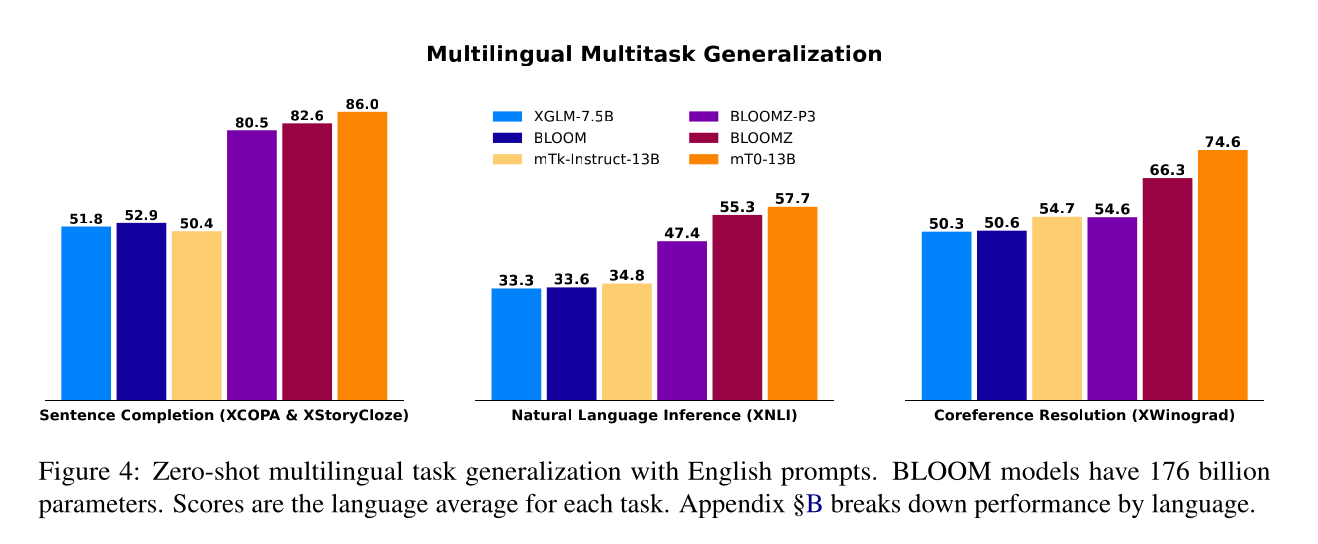
\includegraphics[width=0.8\textwidth]{img/performance_benchmark_bloom.png}
    \caption{Benchmark delle prestazioni di varie versioni di BLOOM}
    \label{fig:performance_benchmark_bloom}
\end{figure}

\subsection{Considerazioni sull'hardware}
Nel caso si volessere utilizzare modelli di grandi dimensioni, come BLOOM, è necessario considerare l'hardware richiesto per l'inferenza. Questi modelli richiedono risorse significative, come GPU ad alte prestazioni e memoria RAM dedicata, per garantire prestazioni ottimali.
Nel nostro caso utilizziamo API endpoint che ci permettono di fare affidamento a risorse cloud per l'inferenza, riducendo la necessità di hardware locale, nel caso dei modelli di Huggingface però, gli API endpoint sono gratuiti solo fino a modelli inferiori ai 10GB, per modelli più grandi è necessario sottoscrivere un piano a pagamento.
\subsubsection{Tabella dei Modelli}
Di seguito è riportata una tabella che elenca i modelli di Huggingface e OpenAI con le loro caratteristiche principali:

\begin{table}[H]
    \centering
    \begin{tabular}{|l|c|c|c|l|}
        \hline
        \textbf{Modello} & \textbf{Parametri} & \textbf{Dimensione (GB)} & \textbf{Hardware Necessario} \\
        \hline
        BLOOM-176B & 176 miliardi & ~350 GB (FP32) & 8x NVIDIA A100 80GB o equivalenti  \\
        \hline
        BLOOM-7.1B & 7,1 miliardi & ~14 GB (FP32) & 1x NVIDIA A100 40GB o equivalenti \\
        \hline
        BLOOM-3B & 3 miliardi & ~6 GB (FP32) & 1x NVIDIA RTX 3090 (24GB) o equivalenti \\
        \hline
        BLOOM-1.1B & 1,1 miliardi & ~2,2 GB (FP32) & 1x NVIDIA RTX 2080 Ti (11GB) o equivalenti \\
        \hline
        BLOOM-560M & 560 milioni & ~1,1 GB (FP32) & 1x NVIDIA GTX 1660 (6GB) o equivalenti \\
        \hline
        BLOOM-350M & 350 milioni & ~0,7 GB (FP32) & 1x GPU integrata con almeno 4GB di memoria \\
        \hline
        BLOOMZ-176B & 176 miliardi & ~350 GB (FP32) & 8x NVIDIA A100 80GB o equivalenti \\
        \hline
        GPT-4o & ~70-100 miliardi & ~140-200 GB (FP32) & 4-8x NVIDIA A100 80GB o equivalenti \\
        \hline
        GPT-4omini & ~3-10 miliardi & ~6-20 GB (FP32) & 1x NVIDIA RTX 3090 (24GB) o equivalenti \\
        \hline
    \end{tabular}
    \caption{Caratteristiche dei modelli di Huggingface e OpenAI}
    \label{tab:modelli}
\end{table}
Bisogna anche considerare il fatto che la dimensione dei modelli non è l'unico fattore determinante per le risorse necessarie, ma anche gli eventuali modelli di embedding e i dataset utilizzati influiscono. È quindi necessario prevedere un margine maggiore per l'hardware utilizzato.
I modelli piccoli come BLOOM-3B o inferiori sono poco efficaci. 

\subsection{OpenAI}
I modelli di OpenAI includono varianti all'avanguardia come GPT-4 e GPT-4omini, sviluppate per fornire elevate prestazioni in una vasta gamma di applicazioni \href{https://code7crusaders.github.io/docs/RTB/documentazione_interna/glossario.html#natural-language-processing-nlp}{NLP\textsuperscript{G}}.

\paragraph*{Caratteristiche principali}
\begin{itemize}
    \item \textbf{Proprietari}: I modelli sono accessibili esclusivamente tramite API commerciali.
    \item \textbf{Prestazioni Elevate}: OpenAI è leader nei benchmark \href{https://code7crusaders.github.io/docs/RTB/documentazione_interna/glossario.html#natural-language-processing-nlp}{NLP\textsuperscript{G}}, garantendo risultati ottimali per applicazioni generative e analitiche.
    \item \textbf{Ottimizzazione per Prodotti Commerciali}: I modelli sono ottimizzati per applicazioni pratiche come chatbot, generazione di codice, automazione aziendale e analisi dei dati.
\end{itemize}

\paragraph*{Vantaggi}
\begin{itemize}
    \item \textbf{Inferenza Scalabile}: Le API cloud di OpenAI permettono una scalabilità elevata senza la necessità di gestione locale delle risorse.
    \item \textbf{Supporto Tecnico}: Documentazione esaustiva e supporto continuo per l'integrazione.
    \item \textbf{Aggiornamenti Regolari}: Miglioramenti costanti ai modelli e alle API.
\end{itemize}

\paragraph*{Svantaggi}
\begin{itemize}
    \item \textbf{Costi Basati sui Token}: I costi dipendono dal numero di token elaborati, il che può risultare oneroso in alcuni scenari ad alto volume.
    \item \textbf{Mancanza di Trasparenza}: Non è possibile accedere ai dati di addestramento o all'architettura interna del modello.
    \item \textbf{Dipendenza dall'Infrastruttura Cloud}: Non è possibile eseguire i modelli localmente, il che può rappresentare un problema per progetti con restrizioni di privacy.
\end{itemize}

\subsubsection{Prestazioni}
\href{https://code7crusaders.github.io/docs/RTB/documentazione_interna/glossario.html#benchmark}{Benchmark\textsuperscript{G}} e valutazione dei modelli di OpenAI: GPT-4o e GPT-4omini, dimostrano prestazioni superiori rispetto ad altri modelli di riferimento.

\begin{figure}[H]
    \centering
    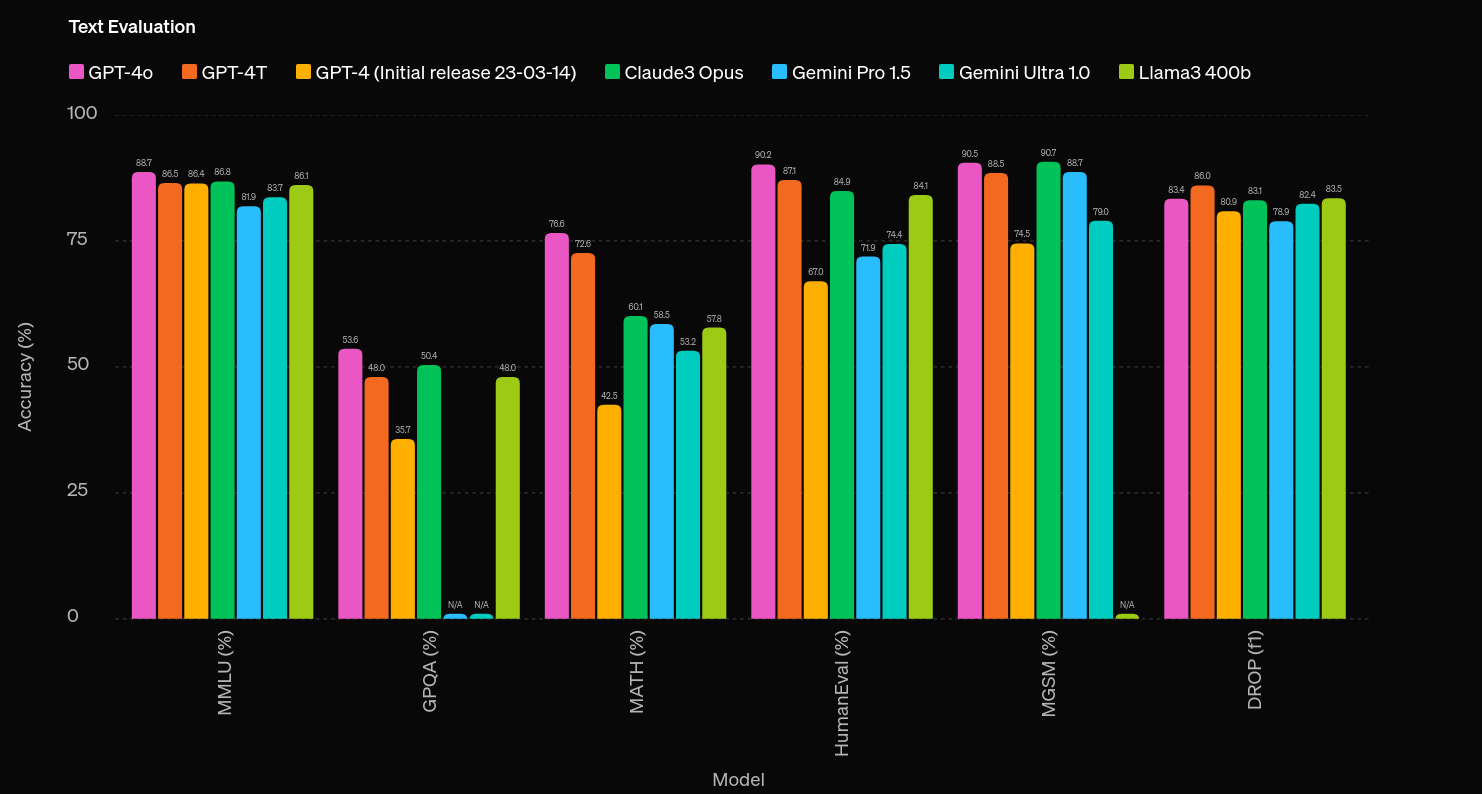
\includegraphics[width=0.8\textwidth]{img/performance_benchmark_gpt4o.png}
    \caption{Benchmark delle prestazioni del modello gpt4o confrontato con altri modelli}
    \label{fig:performance_benchmark_gpt4o}
\end{figure}

\begin{figure}[H]
    \centering
    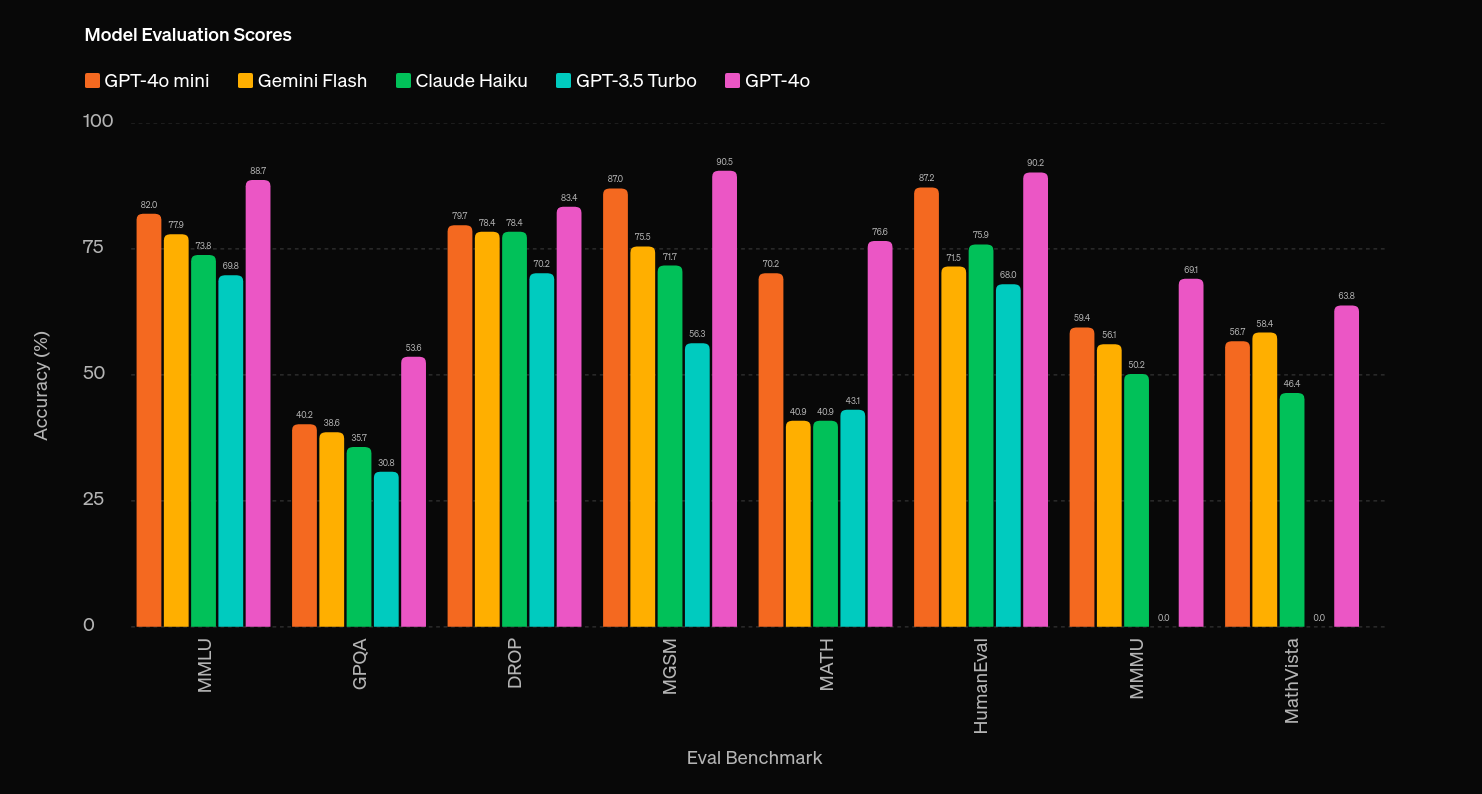
\includegraphics[width=0.8\textwidth]{img/performance_benchmark_gpt4omini.png}
    \caption{Benchmark delle prestazioni del modello gpt4omini confrontato con altri modelli}
    \label{fig:performance_benchmark_gpt4omini}
\end{figure}

\section{Costi e Limiti}
Una differenza chiave tra le due piattaforme riguarda i costi e le limitazioni di utilizzo:

\subsection{Huggingface}
\begin{itemize}
    \item Gli endpoint API di Huggingface supportano modelli fino a 10GB gratuitamente.
    \item Per modelli più grandi è necessario sottoscrivere un piano a pagamento, con costi variabili in base alla dimensione e \textbf{all'utilizzo orario}.
    \item L'utilizzo locale richiede risorse hardware significative, con costi indiretti per l'acquisto o il noleggio di infrastrutture adeguate.
\end{itemize}

\subsubsection{Costi}
Nel nostro caso, data la necessità di utilizzare modelli di grandi dimensioni come BLOOM \textit{(a causa dell'inefficienza di quelli piccoli)}, i costi di Huggingface potrebbero risultare proibitivi,
quindi di seguito mostriamo una tabella che elenca i costi di un API endpoint:

\begin{figure}[H]
    \centering
    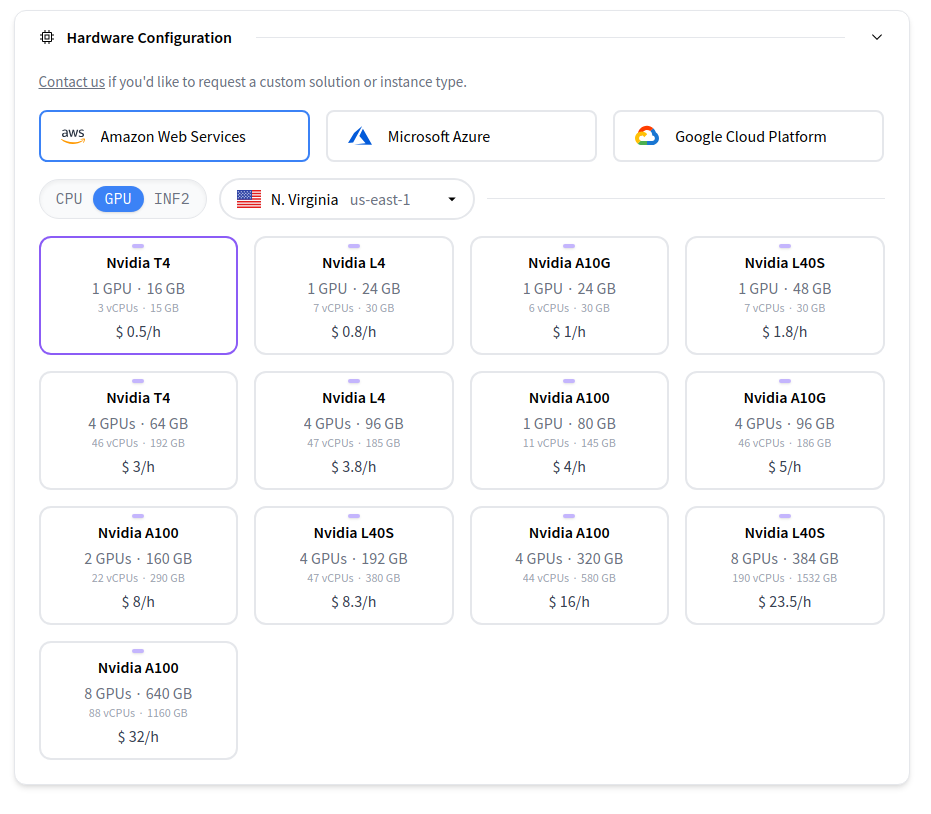
\includegraphics[width=0.8\textwidth]{img/costi_hugginface_api_endpoint.png}
    \caption{Costi degli endpoint API di Huggingface per modelli di grandi dimensioni}
    \label{fig:costi_hugginface_api_endpoint}
\end{figure}




\subsection{OpenAI}
\begin{itemize}
    \item I costi sono calcolati in base al numero di token utilizzati durante l'elaborazione, rendendo il modello economicamente flessibile per casi d'uso specifici.
    \item Non ci sono costi orari fissi, e l'utilizzo è facilmente scalabile in funzione delle esigenze del progetto.
\end{itemize}

Questa differenza rende OpenAI una scelta più conveniente per progetti con utilizzo intermittente o moderato, mentre Huggingface è più adatto a sviluppatori con infrastrutture locali preesistenti o budget elevati per l'acquisto di risorse.

\subsubsection{Costi}
Di seguiti i costi di OpenAI per l'utilizzo delle API per gpt4o e gpt4omini, che a diferrenza di Huggingface non richiedono costi fissi orari ma sono basati sul numero di token utilizzati: 
\begin{figure}[H]
    \centering
    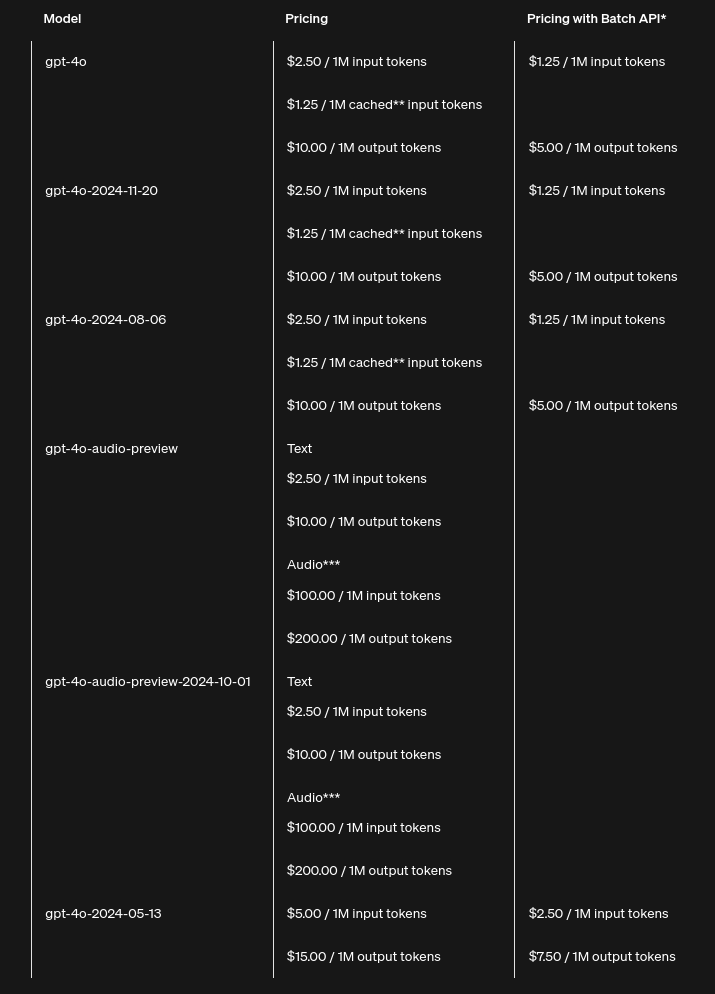
\includegraphics[width=0.8\textwidth]{img/costi_gpt4o.png}
    \caption{Costi delle API di OpenAI per il modello gpt4o}
    \label{fig:costi_openai_gpt4o}
\end{figure}

\begin{figure}[H]
    \centering
    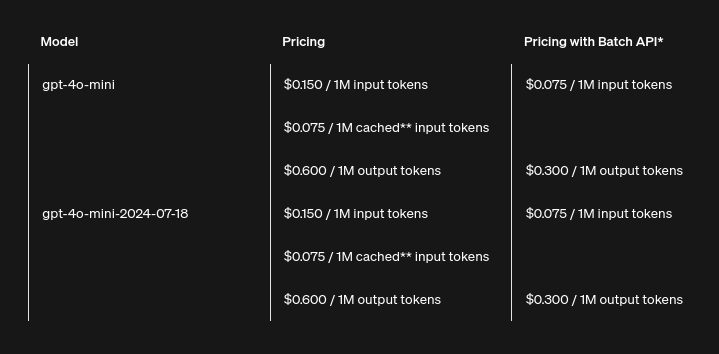
\includegraphics[width=0.8\textwidth]{img/costi_gpt4omini.png}
    \caption{Costi delle API di OpenAI per il modello gpt4omini}
    \label{fig:costi_openai_gpt4omini}
\end{figure}




\section{Utilizzo tramite LangChain}
LangChain è una libreria versatile che consente di combinare modelli linguistici avanzati con strumenti di ricerca, database e altre tecnologie. Entrambe le piattaforme possono essere integrate facilmente tramite LangChain.

\subsection{BigScience Workshop (Huggingface)}
\href{https://code7crusaders.github.io/docs/RTB/documentazione_interna/glossario.html#langchain}{LangChain\textsuperscript{G}} supporta l'integrazione con i modelli Huggingface tramite connettori diretti, permettendo un elevato grado di personalizzazione.

\paragraph*{Punti di forza}
\begin{itemize}
    \item Possibilità di controllare in dettaglio le modalità di esecuzione del modello.
    \item Personalizzazione avanzata per applicazioni specifiche.
\end{itemize}

\paragraph*{Limiti}
\begin{itemize}
    \item Requisiti tecnici e computazionali elevati per ottimizzare le prestazioni.
    \item Gestione complessa per l'utilizzo di modelli di grandi dimensioni.
\end{itemize}

\subsection{OpenAI}
\href{https://code7crusaders.github.io/docs/RTB/documentazione_interna/glossario.html#langchain}{LangChain\textsuperscript{G}} offre un'integrazione nativa con le API di OpenAI, semplificando l'implementazione e l'uso dei modelli.

\paragraph*{Punti di forza}
\begin{itemize}
    \item Configurazione immediata e intuitiva.
    \item Alta scalabilità e tempi di risposta rapidi grazie all'infrastruttura cloud.
\end{itemize}

\paragraph*{Limiti}
\begin{itemize}
    \item Dipendenza dalle API proprietarie.
    \item Costi ricorrenti legati al consumo di token.
\end{itemize}


\section{Testing con OpenAI GPT-4omini e LangChain}
Per valutare l'efficacia dell'integrazione di OpenAI GPT-4omini tramite LangChain, abbiamo condotto una serie di test. Abbiamo utilizzato LangSmith per monitorare le prestazioni e raccogliere dati dettagliati sull'elaborazione.

\subsection{Setup del Test}
Abbiamo configurato un ambiente di test utilizzando \href{https://code7crusaders.github.io/docs/RTB/documentazione_interna/glossario.html#langchain}{LangChain\textsuperscript{G}} per interfacciarci con le API di OpenAI. Il setup includeva:
\begin{itemize}
    \item Un'istanza di \href{https://code7crusaders.github.io/docs/RTB/documentazione_interna/glossario.html#langchain}{LangChain\textsuperscript{G}} configurata per utilizzare GPT-4omini.
    \item Monitoraggio delle richieste e delle risposte tramite LangSmith.
    \item Un istanza RAG (Retrieval-Augmented Generation), realizzata tramite un database vettoriale \href{https://code7crusaders.github.io/docs/RTB/documentazione_interna/glossario.html#faiss}{FAISS\textsuperscript{G}} e come embedding model \href{https://code7crusaders.github.io/docs/RTB/documentazione_interna/glossario.html#bert-bidirectional-encoder-representations-from-transformers}{BERT\textsuperscript{G}}(di Huggingface) runnato in locale(2GB VRAM circa compresi dati file esterni vettorializzati) che ci ha permesso di testare llm su contesti ricevuti da file esterni.
\end{itemize}

\subsection{Esecuzione del Test}
Abbiamo eseguito diversi scenari di test per valutare soprattutto il costo in token dell'utilizzo di GPT-4omini:
\begin{figure}[H]
    \centering
    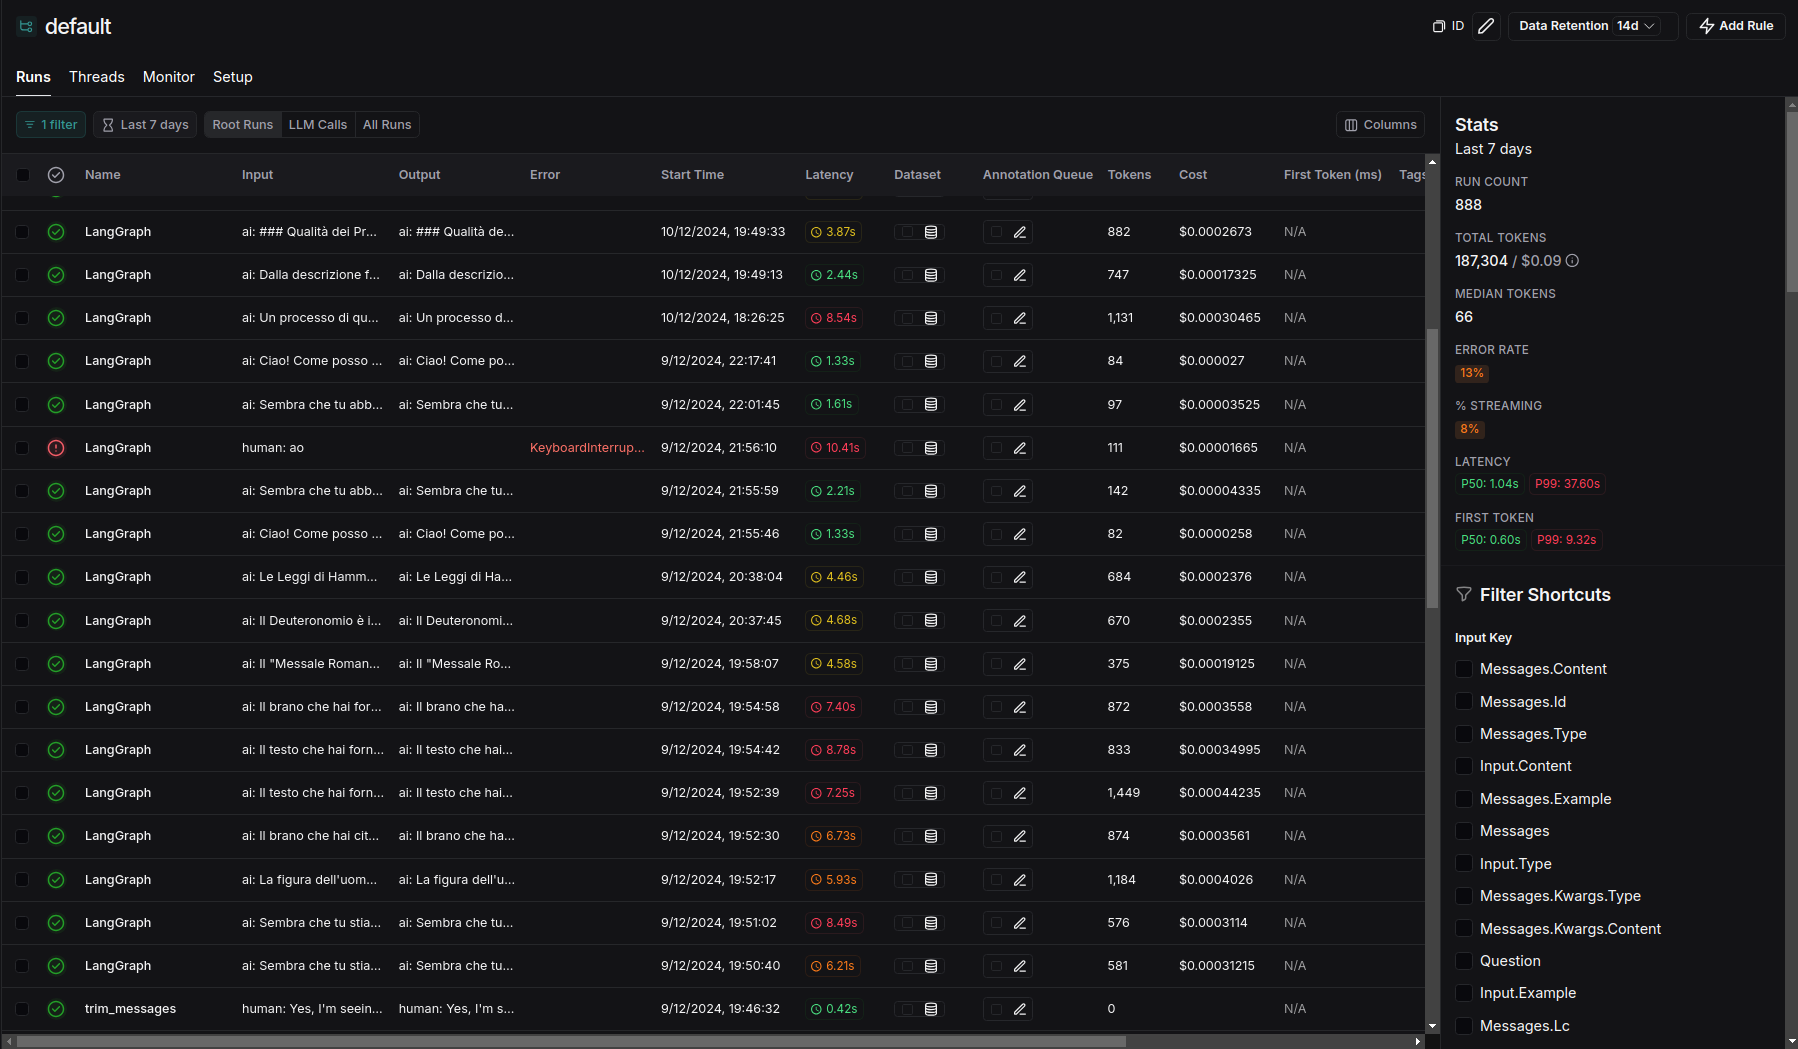
\includegraphics[width=0.8\textwidth]{img/testing_langsmith.png}
    \caption{Scenario riassuntivo dei costi delle varie query su LangSmith}
    \label{fig:LangSmith_costs_summary}
\end{figure}

\subsection{Conclusioni del Test}
I test hanno dimostrato che l'integrazione di GPT-4omini tramite \href{https://code7crusaders.github.io/docs/RTB/documentazione_interna/glossario.html#langchain}{LangChain\textsuperscript{G}} è efficace e offre prestazioni soddisfacenti per le nostre esigenze. Il monitoraggio tramite LangSmith ha fornito dati utili per ottimizzare l'uso del modello e gestire i costi associati all'utilizzo dei token.

In conclusione, l'uso di OpenAI GPT-4omini con \href{https://code7crusaders.github.io/docs/RTB/documentazione_interna/glossario.html#langchain}{LangChain\textsuperscript{G}} rappresenta una soluzione valida per il nostro progetto, garantendo un equilibrio tra prestazioni elevate e costi gestibili.

\section{Conclusioni}
La scelta tra Huggingface e OpenAI dipende dalle esigenze specifiche del progetto e dalle risorse disponibili.

Huggingface è ideale per sviluppatori che richiedono trasparenza, controllo e la possibilità di eseguire modelli su infrastrutture locali. Tuttavia, i costi associati a modelli di grandi dimensioni e le elevate richieste hardware possono rappresentare uno svantaggio.

OpenAI è la soluzione preferibile per applicazioni commerciali o progetti che richiedono elevate prestazioni con un'infrastruttura cloud scalabile e tempi di implementazione rapidi. I costi basati sui token offrono maggiore flessibilità economica rispetto ai costi fissi di Huggingface.

Grazie a LangChain, entrambe le opzioni possono essere integrate efficacemente, permettendo di sfruttare appieno le potenzialità dei modelli linguistici per applicazioni avanzate. 

Tuttavia, per il nostro progetto \textbf{Capitolato 7 Ergon}, l'opzione con OpenAI sembra essere la più adatta all'implementazione pratica, considerati i nostri mezzi e possibilità.

\begin{table}[b]
    \begin{tabular}{@{}p{.5in}p{4in}@{}}
        Data:  & \hrulefill \\
               &     		\\
               &     		\\
        Firma: & \hrulefill \\
    \end{tabular}
    \end{table}


\end{document}
